\documentclass[a4paper]{article}
\usepackage[english]{babel} % English-language report
\usepackage{float} % required for the [H] figure placement option
%\usepackage{simplemargins}

%\usepackage[square]{natbib}
\usepackage{amsmath}
\usepackage{amsfonts}
\usepackage{amssymb}
\usepackage{bbold}
\usepackage{graphicx}
\usepackage{blindtext}
\usepackage{hyperref}
\usepackage{amsthm}
\newtheorem{theorem}{Theorem}
\newtheorem{lemma}{Lemma}
\usepackage{algorithm}
%\usepackage{algorithmic}
\usepackage{algpseudocode}
%\usepackage{algorithm2e}
\usepackage{booktabs}
\usepackage[export]{adjustbox}
\setcounter{MaxMatrixCols}{20}

\begin{document}
\pagenumbering{arabic}

\Large
 \begin{center}
\textbf{Finite Element Method}\\


\hspace{10pt}

% Author names and affiliations
\large
%Lic. Julio A. Medina$^1$ \\
Julio A. Medina\\
\hspace{10pt}
\small  
University of San Carlos of Guatemala\\
School of Physical Sciences and Mathematics\\
Master's Program in Physics\\
\href{mailto:julioantonio.medina@gmail.com}{julioantonio.medina@gmail.com}\\

\end{center}

\hspace{10pt}

\normalsize
\begin{abstract}
This report provides a theoretical introduction to the Finite Element Method (FEM) for solving partial differential equations subject to boundary conditions. It also presents relatively concise implementations for elliptic, parabolic, and hyperbolic partial differential equations. The discussion includes the tessellation, or domain-discretization, process and compares computational implementations in \texttt{Wolfram Mathematica} and \texttt{Python}.
\end{abstract}
\section{Overview of the Finite Element Method}
There are several theoretical approaches to the finite element method. The introduction developed in this document follows a functional approach, in which the objective is to minimize a functional constructed from the specific problem under consideration. This is the approach presented in \cite{Burden}, analogous to the Ritz method.\\
A brief account of the weak formulation is also included. Starting from the partial differential equation, an integral statement is derived that must hold for suitable test functions. This formalism is required to solve the problems with the \texttt{Python} library \texttt{FEniCS}. Both approaches are rooted in the calculus of variations.
\section{Introduction to the Finite Element Method}
This method for approximating solutions of partial differential equations was originally developed for civil-engineering applications. It is now used throughout applied mathematics and in many areas of physics. FEM is employed extensively in the modeling of complex systems, the aerodynamic design of components, space-exploration technology, and advanced engineering applications such as Formula One racing.\\

One advantage of the finite element method over the finite difference method is the relative ease with which FEM handles boundary conditions. Many physical problems have boundary conditions involving derivatives and irregular boundaries without apparent symmetries. Such conditions can be difficult to treat with finite differences because every derivative boundary condition must be approximated by a difference quotient at grid points, while irregular boundaries make the construction of a suitable grid nontrivial. In FEM, boundary conditions can instead enter through the variational formulation, so the overall construction is better suited to irregular geometries and mixed boundary conditions.\\

The partial differential equation considered is
\begin{equation}\label{eq::partial_diff_equation}
\frac{\partial}{\partial x}\Bigg( p(x,y)\frac{\partial u}{\partial x} \Bigg) + \frac{\partial}{\partial y}\Bigg( q(x,y)\frac{\partial u}{\partial y} \Bigg) +r(x,y)u(x,y)=f(x,y)
\end{equation}
for $(x,y)\in \mathcal{D}$, where $\mathcal{D}$ is a planar region with boundary $\mathcal{S}$.\\

Boundary conditions of the form
\begin{equation}\label{eq::boundary1}
u(x,y)=g(x,y)
\end{equation}
are imposed on a portion $\mathcal{S}_1$ of the boundary. On the remaining portion, $\mathcal{S}_2$, the solution is required to satisfy
\begin{equation}\label{eq:boundary2}
p(x,y)\frac{\partial u}{\partial x}(x,y)\cos\theta_1+q(x,y)\frac{\partial u}{\partial y}(x,y)\cos\theta_2+g_1(x,y)u(x,y)=g_2(x,y),
\end{equation}
where $\theta_1$ and $\theta_2$ are the direction angles of the outward normal at the point $(x,y)$; see Figure \ref{fig::fig1}.
\begin{figure}[h]
\begin{center}
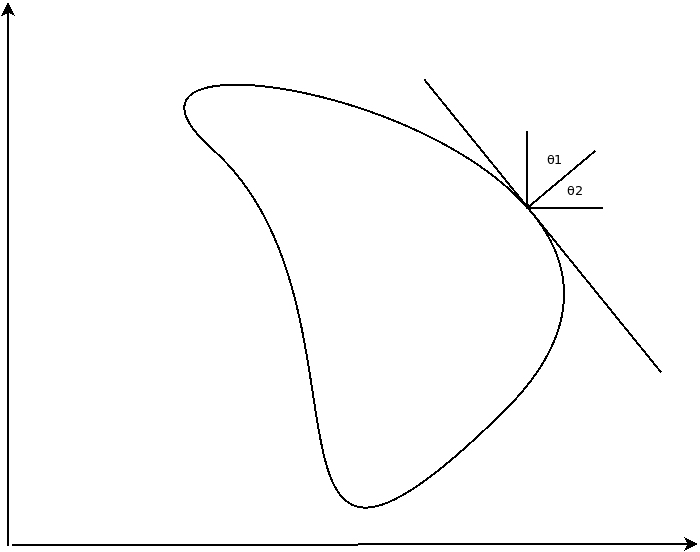
\includegraphics[scale=0.42]{../report/fig1.png} 
\end{center} 
\caption{Direction angles $\theta_1$ and $\theta_2$}
\label{fig::fig1}
\end{figure}
Physical problems in areas such as solid mechanics and elasticity often involve partial differential equations similar to \ref{eq::partial_diff_equation}. Their solutions typically minimize a functional involving definite integrals over a class of functions determined by the problem.\\

Assume that $p,q,r$, and $f$ are continuous on $\mathcal{D}\cup\mathcal{S}$; that $p$ and $q$ have continuous first partial derivatives; and that $g_1$ and $g_2$ are continuous on $\mathcal{S}_2$. In addition, assume that $p(x,y)>0$, $q(x,y)>0$, $r(x,y)\leq 0$, and $g_1(x,y)>0$. Then the solution of \ref{eq::partial_diff_equation} is the unique minimizer of the functional $I[w]$.
\begin{equation}\label{eq::functional}
\begin{aligned}
I[w]=\int\int_{\mathcal{D}}\Bigg\{ \frac{1}{2}\Big[p(x,y)\Big( \frac{\partial w}{\partial x} \Big)^2 + q(x,y)\Big( \frac{\partial w}{\partial y} \Big)^2 -r(x,y) w^2 \Big] +f(x,y)w\Bigg\}dx dy\\
+\int_{\mathcal{S}_2}\Bigg\{ -g_2(x,y)w+\frac{1}{2}g_1(x,y)w^2 \Bigg\}dS
\end{aligned}
\end{equation}
over all twice-differentiable continuous functions $w$ that satisfy \ref{eq::boundary1} on $\mathcal{S}_1$. The finite element method approximates this solution by minimizing the functional $I$ in \ref{eq::functional} over a smaller finite-dimensional class of functions, similarly to the Rayleigh--Ritz approach; see \cite{Burden}.
\subsection{Defining the Finite Elements}
The first step is to define the finite elements used to construct the approximation. The region is divided into a finite number of regularly shaped sections or elements, such as triangles or rectangles, that tessellate and discretize the entire domain.\\

The approximation space is commonly formed by piecewise polynomials of fixed degree in $x$ and $y$. The pieces are joined so that the resulting function is continuous and has the required weak derivatives over the whole region. Linear polynomials in $x$ and $y$ of the form
\begin{equation}
\phi(x,y)=a+bx+cy
\end{equation}
are commonly used with triangular elements, whereas bilinear polynomials in $x$ and $y$ of the form
\begin{equation}
\phi(x,y)=a+bx+cy+dxy
\end{equation}
are associated with rectangular elements.\\

Assume that the region $\mathcal{D}$ has been subdivided into triangular elements. Let $D$ denote the collection of triangles, whose vertices are called nodes. The method seeks an approximation of the form
\begin{equation}
\phi(x,y)=\sum_{i=1}^{m}\gamma_i \phi_i(x,y),
\end{equation}
where $\phi_1,\phi_2,\hdots,\phi_m$ are linearly independent piecewise-linear polynomials and $\gamma_1,\gamma_2,\hdots,\gamma_m$ are constants. Some of these constants, for example $\gamma_{n+1},\gamma_{n+2},\hdots,\gamma_m$, are used to enforce the boundary condition
\begin{equation}\label{eq::phi}
\phi(x,y)=g(x,y)
\end{equation}
on $\mathcal{S}_1$. The remaining constants $\gamma_1,\gamma_2,\hdots,\gamma_n$ are chosen to minimize $I[\sum_{i=1}^m \gamma_i\phi_i]$. Substituting the approximation \ref{eq::phi} for $w$ in \ref{eq::functional} gives
\begin{equation}\label{eq::aproximated_functional}
\begin{aligned}
I[\phi]&=I\Big[ \sum_{i=1}^{m} \gamma_i \phi_i \Big]\\
&=\int\int_{\mathcal{D}}\Bigg(\frac{1}{2}\Bigg\{ p(x,y)\Big[ \sum_{i=1}^{m}\gamma_i \frac{\partial \phi_i}{\partial x}(x,y)\Big]^2 + q(x,y)\Big[ \sum_{i=1}^{m}\gamma_i \frac{\partial \phi_i}{\partial y}(x,y)\Big]^2\\
&-r(x,y)\Big[ \sum_{i=1}^{m}\gamma_i \phi_i(x,y)\Big]^2\Bigg\}+f(x,y)\sum_{i=1}^m \gamma_i \phi_i(x,y)\Bigg)dy\, dx\\
&\quad +\int_{\mathcal{S}_2}\Bigg\{ -g_2(x,y)\sum_{i=1}^m \gamma_i \phi_i(x,y)+\frac{1}{2}g_1(x,y)\Big[\sum_{i=1}^m \gamma_i \phi_i(x,y)\Big]^2\Bigg\}dS
\end{aligned}
\end{equation}
As noted above, $\gamma_1,\gamma_2,\hdots,\gamma_n$ are selected to minimize the functional. Treating $I$ as a function $I[\gamma_1,\gamma_2,\hdots,\gamma_n]$, a necessary condition for a minimum is
\begin{equation}\label{eq::minimun_condition}
\frac{d I}{d \gamma_j}=0,\,\, \forall\, j=1,2,\hdots,n.
\end{equation}

Differentiating \ref{eq::aproximated_functional} with respect to $\gamma_j$ gives
\begin{equation}
\begin{aligned}
\frac{\partial I}{\partial \gamma_j}=&\int \int_{\mathcal{D}}\Bigg\{p(x,y)\sum_{i=1}^m \gamma_i\frac{\partial \phi_i}{\partial x}(x,y)\frac{\partial \phi_j}{\partial x}(x,y)\\
& + q(x,y)\sum_{i=1}^{m}\gamma_i\frac{\partial \phi_i}{\partial y}(x,y)\frac{\partial \phi_j}{\partial y}(x,y)\\
& - r(x,y)\sum_{i=1}^{m}\gamma_i \phi_i(x,y)\phi_j(x,y)+f(x,y)\phi_j(x,y)\Bigg\}dx\,dy\\
& + \int_{\mathcal{S}_2}\Bigg\{-g_2(x,y)\phi_j(x,y)+g_1(x,y)\sum_{i=1}^m \gamma_i \phi_i(x,y)\phi_j(x,y)\Bigg\}dS,
\end{aligned}
\end{equation}
and therefore the stationarity condition becomes
\begin{equation}
\begin{aligned}
0&=\sum_{i=1}^m \Bigg[\int \int_{\mathcal{D}}\Bigg\{ p(x,y)\frac{\partial \phi_i}{\partial x}(x,y)\frac{\partial \phi_j}{\partial x}(x,y)+ q(x,y)\frac{\partial \phi_i}{\partial y}(x,y)\frac{\partial \phi_j}{\partial y}(x,y)\\
&-r(x,y)\phi_i(x,y)\phi_j(x,y)\Bigg\}dx\,dy\\
&+ \int_{\mathcal{S}_2}g_1(x,y)\phi_i(x,y)\phi_j(x,y)dS\Bigg]\gamma_i\\
&+ \int\int_{\mathcal{D}} f(x,y)\phi_j(x,y)dx\,dy-\int_{\mathcal{S}_2} g_2(x,y)\phi_j(x,y)dS.
\end{aligned}
\end{equation}
for each $j=1,2,\hdots,n$. This system of equations can be written in matrix form as
\begin{equation}
\mathbf{A}\vec{c}=\vec{b},
\end{equation}
where $\vec{c}=(\gamma_1,\hdots,\gamma_n)^t$. The matrix $\mathbf{A}=(\alpha_{ij})$ and vector $\vec{b}=(\beta_1,\hdots,\beta_n)^t$ are defined below.
\begin{equation}\label{eq::alpha_ij}
\begin{aligned}
\alpha_{ij}=\int\int_{\mathcal{D}}\Bigg[ p(x,y)\frac{\partial \phi_i}{\partial x}(x,y)\frac{\partial \phi_j}{\partial x}(x,y)+ q(x,y)\frac{\partial \phi_i}{\partial y}(x,y)\frac{\partial \phi_j}{\partial y}(x,y)\\
-r(x,y)\phi_i(x,y)\phi_j(x,y)\Bigg] dx\,dy+\int_{\mathcal{S}_2} g_1(x,y)\phi_i(x,y)\phi_j(x,y)dS,
\end{aligned}
\end{equation}
for each $i=1,2,\hdots,n$ and $j=1,2,\hdots,m$, and
\begin{equation}\label{eq::beta_i}
\beta_i=-\int\int_{\mathcal{D}}f(x,y)\phi_i(x,y) dx\,dy+\int_{\mathcal{S}} g_2(x,y)\phi_i(x,y)dS-\sum_{k=n+1}^m\alpha_{ik}\gamma_k.
\end{equation}
for each $i=1,\hdots,n$.\\

The choice of basis functions is important because an appropriate selection can often make $\mathbf{A}$ positive definite and give it a banded-matrix structure. For the second-order problem \ref{eq::partial_diff_equation}, the domain $\mathcal{D}$ is assumed to be polygonal, so that $\mathcal{D}=D$, and $\mathcal{S}$ is a set of contiguous straight-line segments.

\subsection{Triangulating the Region}
To begin the procedure described above, the region $D$ must be subdivided into triangles $T_1,T_2,\hdots,T_M$. Triangle $i$ has three vertices, or nodes, denoted by
\begin{equation}\label{eq::triangle_vertex}
V_j^{(i)}=\big( x_j^{(i)},y_j^{(i)} \big),\,\,\, \text{for }\, j=1,2,3.
\end{equation}
For simplicity, write $V_j^{(i)}=\big(x_j^{(i)},y_j^{(i)}\big)$ while working with a fixed triangle $T_i$. Associated with each vertex $V_j$ is a linear polynomial
\begin{equation}
N_j^{(i)}(x,y)\equiv N_j(x,y)=a_j+b_jx+c_jy,\,\,\,\text{where }\, N_j^{(i)}(x_k,y_k)=
\begin{cases}
1, & j=k\\
0, & j\neq k
\end{cases}
\end{equation}
This construction produces a linear system of the form
\begin{equation}\label{eq::vertex_equation}
\begin{bmatrix}
1 & x_1 & y_1\\
1 & x_2 & y_2\\
1 & x_3 & y_3
\end{bmatrix}
\begin{bmatrix}
a_j\\
b_j\\
c_j
\end{bmatrix}=
\begin{bmatrix}
0\\
1\\
0
\end{bmatrix}.
\end{equation}
In \ref{eq::vertex_equation}, $j=2$, so the entry equal to $1$ occurs in row 2. In general, the entry equal to $1$ occurs in row $j$.\\

Suppose that the nodes $E_1,\hdots,E_n$ in $D\cap\mathcal{S}$ have been labeled. Each node $E_k$ is associated with a function $\phi_k$ that is linear on every triangle, equals $1$ at $E_k$, and equals $0$ at every other node. This construction makes $\phi_k$ identical to $N_j^{(i)}$ on triangle $T_i$ whenever $E_k$ is the vertex denoted by $V_j^{(i)}$.

\section{Weak Formulation for FEM}
The discussion begins with the original problem, also known as the strong formulation. Consider the elliptic partial differential equation given by the Poisson equation
\begin{equation}\label{eq::strong_form}
\nabla^2 T= f(x)
\end{equation}
with the Dirichlet condition
\begin{equation}
T=u(x), \,\,\,\,x\in \Gamma_D
\end{equation}
and the Neumann condition
\begin{equation}
\nabla T \cdot \mathbf{n}=g(x),\,\,\,x\in \Gamma_N
\end{equation}
where $\Omega\subset\mathbb{R}^n$ is the solution domain with boundary $\partial\Omega$, $\Gamma_D$ is the portion of the boundary on which the Dirichlet condition is imposed, and $\Gamma_N$ is the portion with a Neumann condition. The function $T(x)$ is the unknown to be found or approximated, while $f(x)$, $u(x)$, and $g(x)$ are known functions.\\
The weak form of \ref{eq::strong_form} is obtained by requiring
\begin{equation}
\int_{\Omega}(\nabla^2 T -f)\cdot s\, d\Omega=0
\end{equation}
where $s$ is a test function. Integration by parts gives
\begin{equation}
\begin{aligned}
0&=\int_{\Omega}(\nabla^2 T -f)\cdot s\, d\Omega=\int_{\Omega}\nabla\cdot\big( \nabla T \big)\cdot s\, d\Omega-\int_{\Omega}f\cdot s d\Omega=\\
&=-\int_{\Omega}\nabla T \cdot \nabla s \,d\Omega + \int_{\Omega}\nabla\cdot\big(\nabla T \cdot s  \big)\,d\Omega-\int_{\Omega} f\cdot s\, d\Omega
\end{aligned}
\end{equation}
Applying the divergence theorem yields
\begin{equation}
\int_{\Omega}\nabla T \cdot \nabla s\,d\Omega = \int\limits_{\Gamma_D \cup \Gamma_N} s\,(\nabla T\cdot \mathbf{n})\,d\Gamma-\int_{\Omega}f\,s\,d\Omega
\end{equation}
The boundary integral can be separated into a contribution from the Dirichlet portion and another from the Neumann portion:
\begin{equation}\label{eq::intial_weak_form}
\int_{\Omega}\nabla T \cdot \nabla s\, d\Omega = \int\limits_{\Gamma_D} s\,(\nabla T\cdot \mathbf{n})\, d\Gamma+\int\limits_{\Gamma_N} s\,(\nabla T\cdot \mathbf{n})\, d\Gamma-\int_{\Omega}f\,s\, d\Omega
\end{equation}
Equation \ref{eq::intial_weak_form} is the initial weak form of the Poisson equation, but it cannot be applied directly without first accounting for the boundary conditions.

\subsection{Dirichlet Boundary Conditions}
On the portion of the boundary where Dirichlet conditions apply, there are two constraints: the boundary condition $T(x)=u(x)$ and the boundary integral over $\Gamma_D$ in \ref{eq::intial_weak_form}. To eliminate that boundary-integral term while enforcing the prescribed value, take $T\in V(\Omega)$ and the test function $s\in V_0(\Omega)$, where
\begin{equation*}
\begin{aligned}
V(\Omega)=\{ &v(x)\in H^1(\Omega)\},\\
V_0(\Omega)=\{v(x) \in& H^1(\Omega);\, v(x)=0,\, x\in\Gamma_D\}.
\end{aligned}
\end{equation*}
In Sobolev-space terms, the unknown $T$ and the test function $s$ belong to $H^1(\Omega)$, so they and their first weak derivatives are square integrable. In addition, the test function vanishes on $\Gamma_D$.\\
With this requirement, the boundary term over $\Gamma_D$ vanishes. The weak form of the Poisson equation for $T\in V(\Omega)$ and $s\in V_0(\Omega)$ is
\begin{equation}
\begin{aligned}
\int_{\Omega}\nabla T\cdot\nabla s\,d\Omega = \int\limits_{\Gamma_N} s\,(\nabla T\cdot\mathbf{n})\,d\Gamma-\int_{\Omega}f\,s\,d\Omega\\
T(x)=u(x),\,\,\, x\in \Gamma_D.
\end{aligned}
\end{equation}
For this reason, Dirichlet conditions are called \textit{essential boundary conditions} in FEM terminology: they are not incorporated automatically by the weak formulation and must be imposed explicitly.
\subsection{Neumann Boundary Conditions}
Neumann boundary conditions prescribe the flux $g(x)=\nabla T\cdot\mathbf{n}$. The boundary integral over $\Gamma_N$ in \ref{eq::intial_weak_form} contains exactly this flux, so $g(x)$ can be substituted directly into the integral:
\begin{equation}
\int_{\Omega} \nabla T\cdot \nabla s \, d\Omega= \int_{\Gamma_N}g\cdot s \, d\Gamma-\int_{\Omega}f\cdot s\,d\Omega,
\end{equation}
where the test function $s$ also belongs to $V_0$.\\
Neumann conditions are therefore called \textit{natural boundary conditions}, because they appear naturally in the weak formulation.
\subsection{Weak Formulation of the Poisson Equation}
Combining the previous results gives the weak formulation of the Poisson equation \ref{eq::strong_form}: for every test function $s\in V_0(\Omega)$, find $T\in V(\Omega)$ such that
\begin{equation}
\begin{aligned}\label{eq::Poisson_weak_formulation}
\int_{\Omega} \nabla T\cdot \nabla s \, d\Omega= \int_{\Gamma_N}g\cdot s \, d\Gamma-\int_{\Omega}f\cdot s\,d\Omega,\\
T(x)=u(x),\,\,\,x\in\Gamma_D.
\end{aligned}
\end{equation}
\section{Implementation Analysis}
This section analyzes finite element implementations in \textbf{Wolfram Mathematica 12} and \textbf{Python}, using the \textbf{FEniCS} library in the latter case; see \cite{FEniCS}. Three classes of partial differential equations are considered:
\begin{itemize}
\item Elliptic equation
\item Hyperbolic equation
\item Parabolic equation

\end{itemize}
\subsection{Elliptic Equation}
The elliptic partial differential equation to be solved is
\begin{equation}\label{eq::elliptic_pde}
\begin{aligned}
\nabla^2 u(x,y)&=x e^y\\
\frac{\partial ^2 u}{\partial x^2}+\frac{\partial ^2 u}{\partial y^2}&=x e^y, \,\,\, 0<x<2,\,\,0<y<1
\end{aligned}
\end{equation}
with boundary conditions
\begin{equation}
\begin{aligned}
u(0,y)=0,\,\,\,u(2,y)=2e^y,\,\,\,0\leq y\leq 1,\\
u(x,0)=x,\,\,\,u(x,1)=ex,\,\,\,0\leq x\leq 2.
\end{aligned}
\end{equation}
This elliptic PDE is the well-known Poisson equation, here considered in two spatial dimensions.\\
\subsubsection{Implementation in Mathematica}
Solving \ref{eq::elliptic_pde} with the \texttt{Needs["NDSolve`FEM`"]} package in \texttt{Wolfram Mathematica 12} gives a numerical solution that can be visualized as a surface embedded in three-dimensional space.
\begin{figure}[H]
\begin{center}
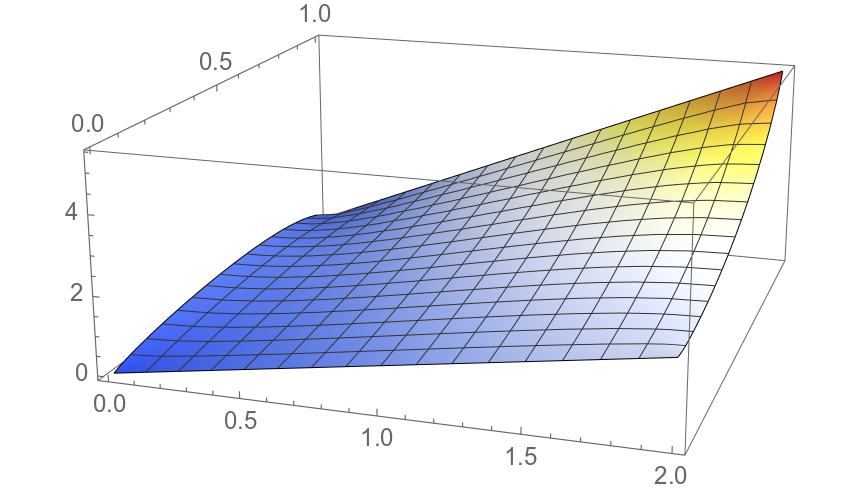
\includegraphics[scale=0.42]{../report/elliptic.png} 
\end{center} 
\caption{Numerical solution of the elliptic PDE}
\label{fig::fig2}
\end{figure}
To demonstrate the geometric capabilities of Mathematica\'s finite element tools, consider solving the elliptic equation on the rectangular region defined above while excluding the points inside the circle described by
\begin{equation}\label{eq::region1}
(x-0.2)^2+(y-0.2)^2\leq 0.3^2
\end{equation}
This produces the following planar region:
\begin{figure}[H]
\begin{center}
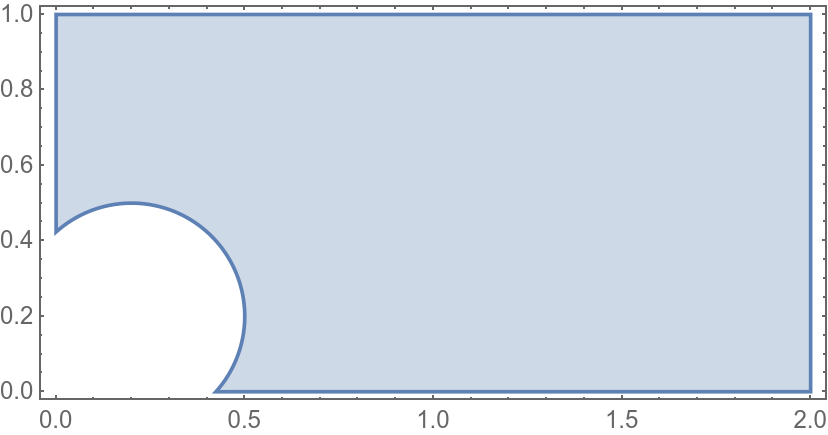
\includegraphics[scale=0.42]{../report/elliptic_omega.png} 
\end{center} 
\caption{Region excluding the points described by \ref{eq::region1}}
\label{fig::elliptic_region}
\end{figure}
In addition to making the region more complex, impose Dirichlet conditions of the form
\begin{equation}
u(x,y)=
\begin{cases}
0, & x=2,\quad 0.8\leq y \leq 1.0\\
10, & (x-0.2)^2+(y-0.2)^2\leq 0.3^2
\end{cases}
\end{equation}
Solving the problem gives the following contour lines:
\begin{figure}[H]
\begin{center}
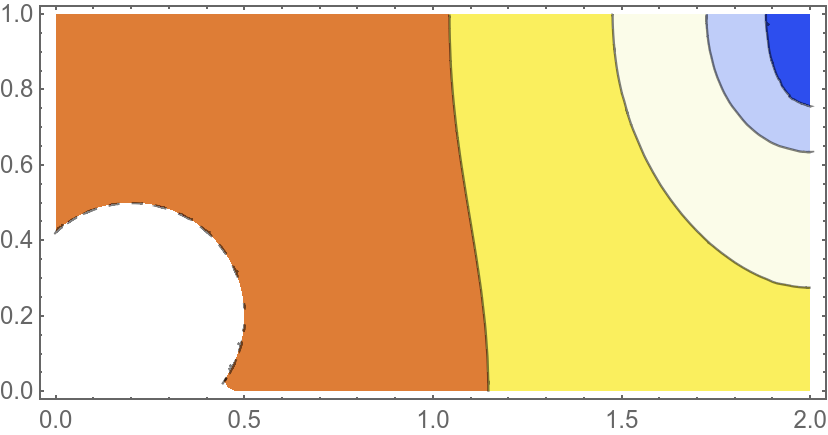
\includegraphics[scale=0.42]{../report/elliptic_omega_contour.png} 
\end{center} 
\caption{Contour lines}
\label{fig::elliptic_contours}
\end{figure}
The corresponding solution in three-dimensional space is shown below.
\begin{figure}[h]
\begin{center}
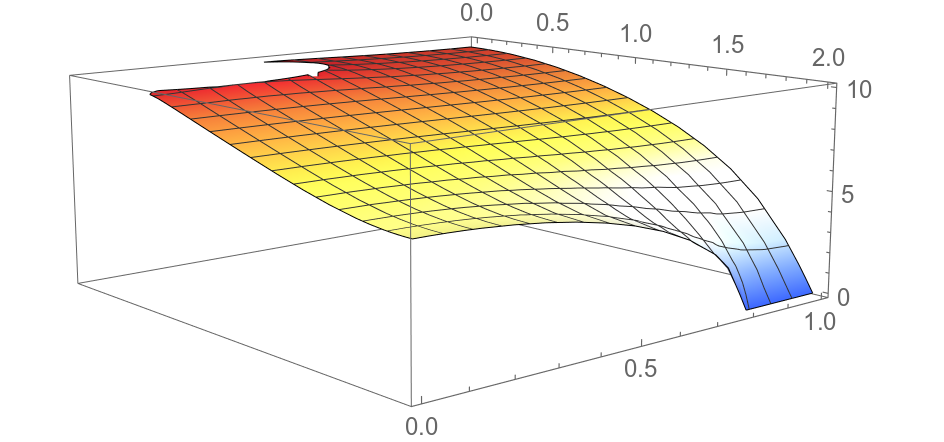
\includegraphics[scale=0.42]{../report/elliptic_omega_3D.png} 
\end{center} 
\caption{Numerical solution with Dirichlet boundary conditions}
\label{fig::elliptic_3d}
\end{figure}
The tessellation of the domain generated by the finite element package can also be visualized:
\begin{figure}[H]
\begin{center}
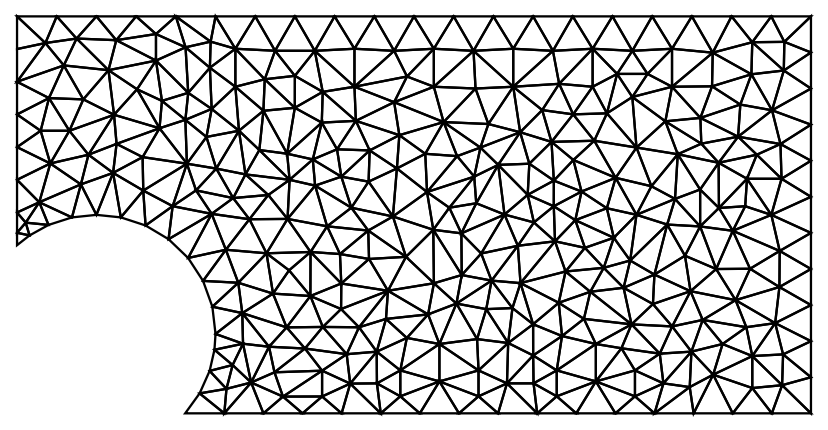
\includegraphics[scale=0.42]{../report/elliptic_omega_mesh.png} 
\end{center} 
\caption{Tessellation of the domain}
\label{fig::elliptic_mesh}
\end{figure}
\subsubsection{Implementation in FEniCS}
To use \texttt{FEniCS}, the PDE must be written in weak form. As discussed above, the terms in \ref{eq::Poisson_weak_formulation} can be used to express the elliptic, or Poisson, problem in code.\\
Applying this procedure to \ref{eq::elliptic_pde} gives the following approximation:
\begin{figure}[H]
\begin{center}
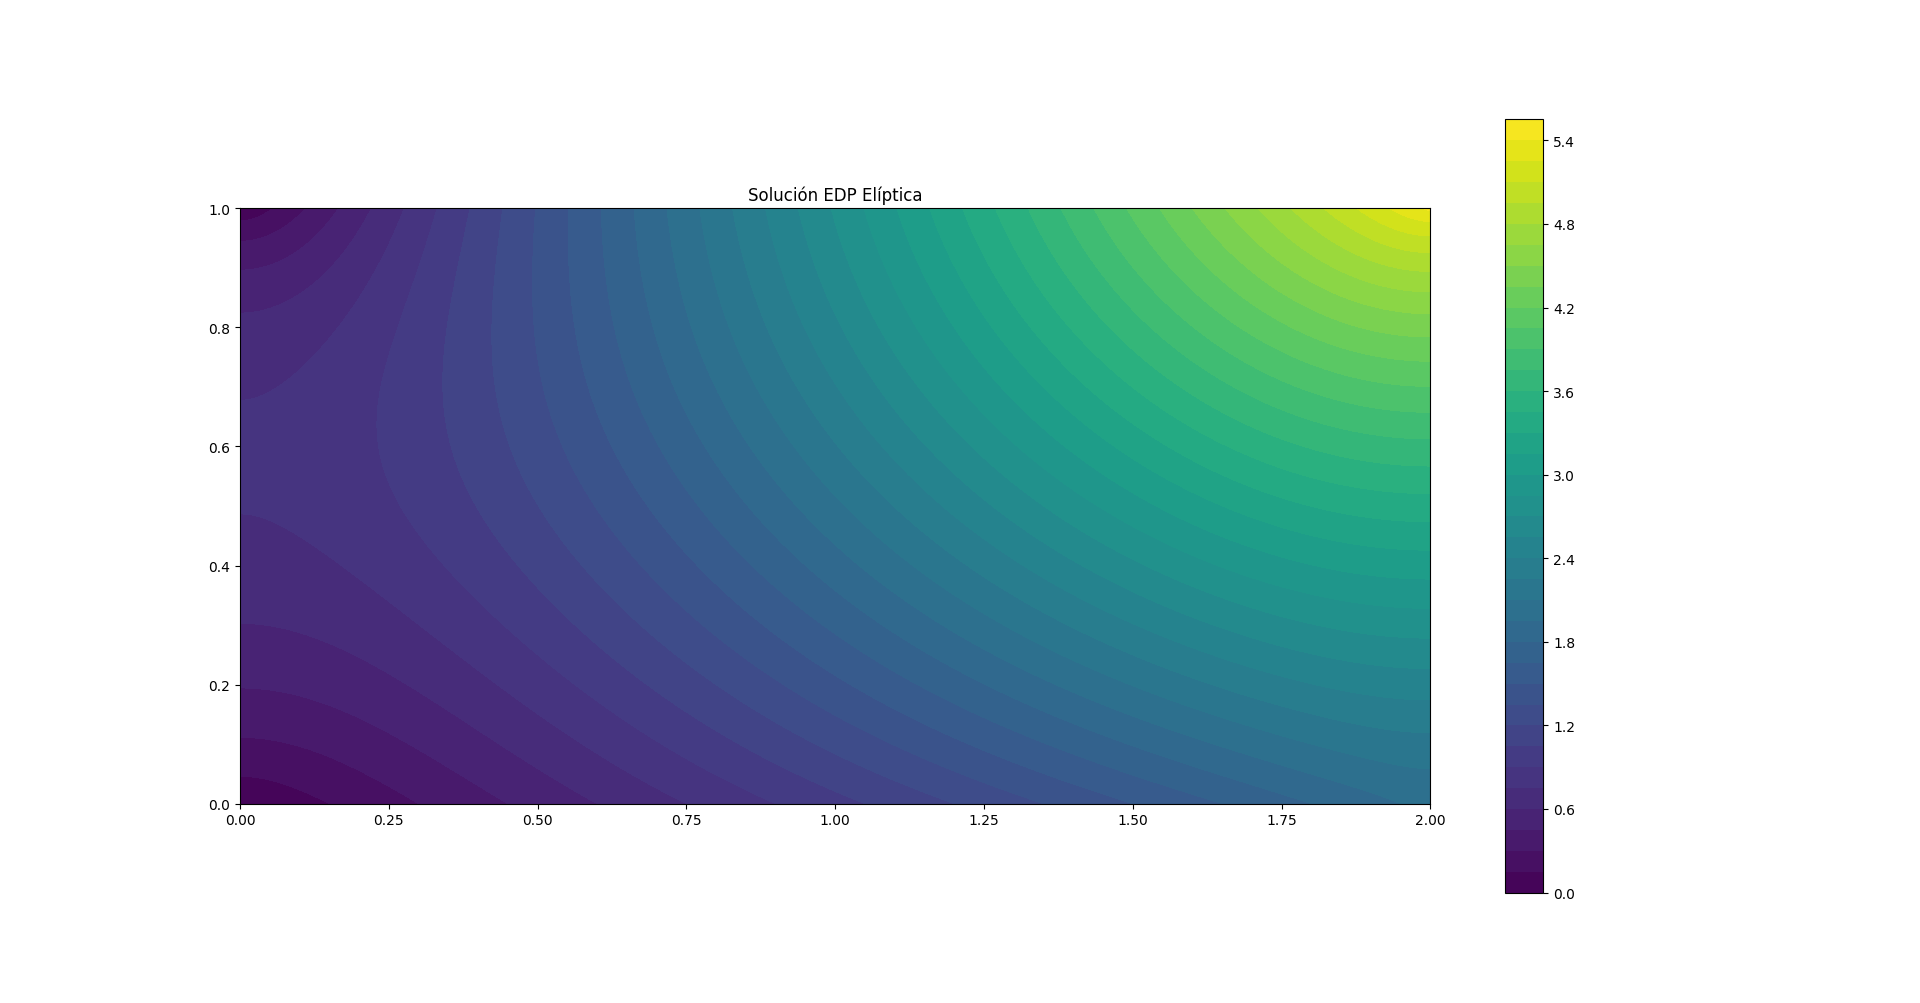
\includegraphics[scale=0.3]{../report/elliptic_FEniCS.png} 
\end{center} 
\caption{Numerical solution of the Poisson equation}
\label{fig::elliptic_fenics}
\end{figure}


\subsection{Parabolic Equation}
For the parabolic equation, consider the problem
\begin{equation}\label{eq::parabolic_pde}
\frac{\partial u}{\partial t}(x,t)-\frac{\partial^2 u}{\partial x^2}(x,t)=0,\,\,\,\,0<x<1,\,\,\,t\geq 0
\end{equation}
with boundary conditions
\begin{equation}
u(0,t)=u(1,t)=0,\,\,\,t>0
\end{equation}
and initial condition
\begin{equation}
u(x,0)=\sin(\pi x),\,\,\, 0 \leq x \leq 1
\end{equation}
\subsubsection{Implementation in Mathematica}
Using \texttt{Needs["NDSolve`FEM`"]} and \texttt{NDSolveValue}, the PDE and its initial and boundary conditions can be specified directly. The numerical approximation is shown below.
\begin{figure}[H]
\begin{center}
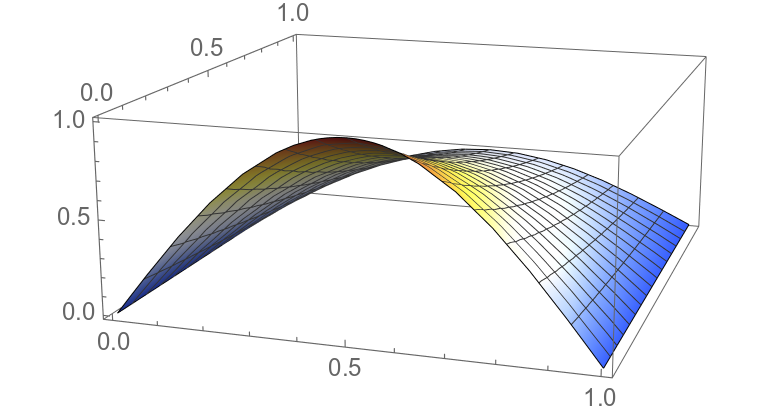
\includegraphics[scale=0.42]{../report/parabolic.png} 
\end{center} 
\caption{Numerical approximation of the parabolic PDE}
\label{fig::parabolic_mathematica}
\end{figure}
It is also useful to visualize the contour lines of the approximate numerical solution.
\begin{figure}[H]
\begin{center}
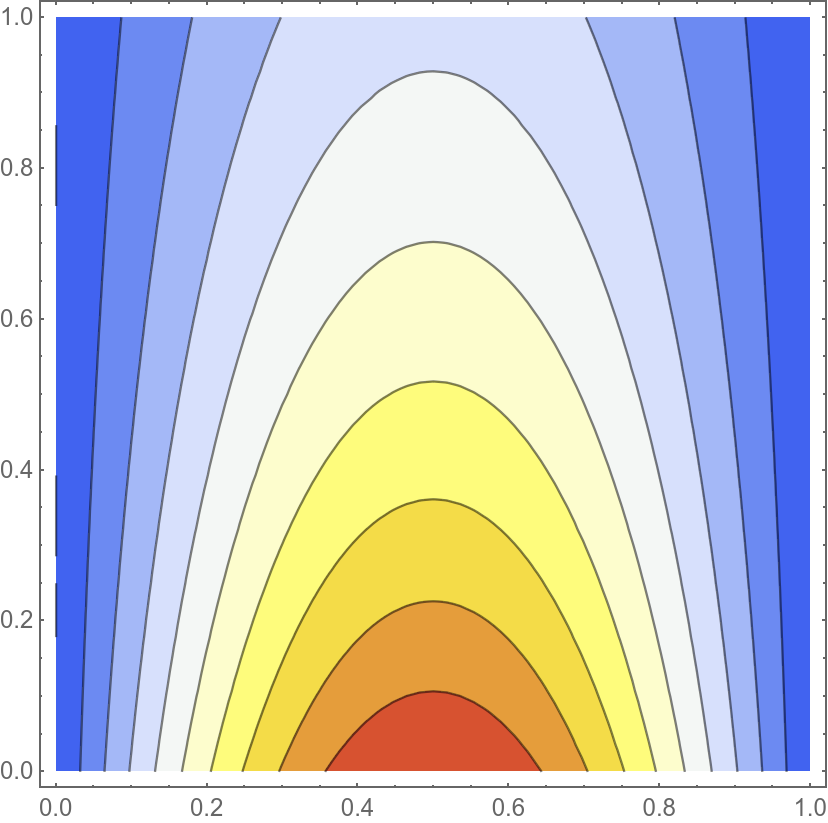
\includegraphics[scale=0.29]{../report/parabolic_contour.png} 
\end{center} 
\caption{Contour lines of the numerical approximation to the parabolic PDE}
\label{fig::parabolic_contours}
\end{figure}
\subsubsection{Implementation in FEniCS}
To solve the equation numerically, the weak form of \ref{eq::parabolic_pde} must be constructed. The corresponding \texttt{Python} code is available in this repository; see \url{https://github.com/Julio-Medina/Finite_Element_Method}.\\
The result obtained with FEniCS is shown below.
\begin{figure}[H]
\begin{center}
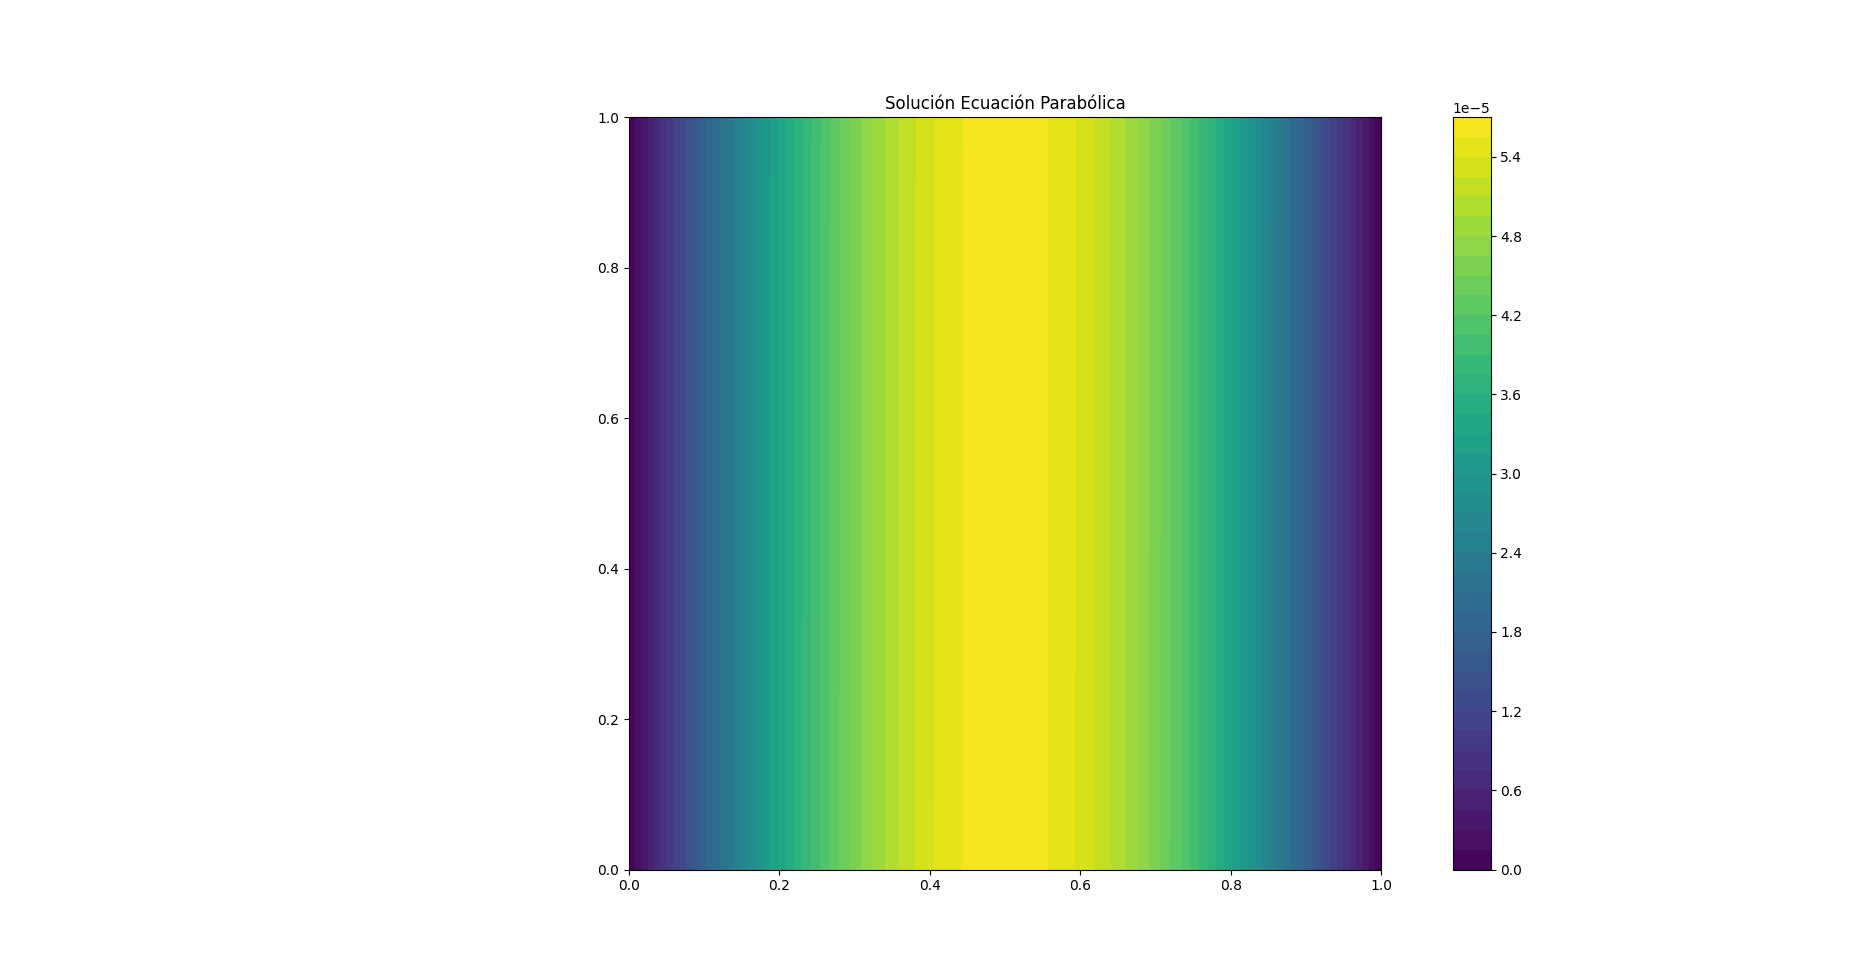
\includegraphics[scale=0.25]{../report/parabolic_FEniCS.png} 
\end{center} 
\caption{Approximation to the solution of the parabolic PDE}
\label{fig::parabolic_fenics}
\end{figure}
The mesh produced by \texttt{FEniCS} can be plotted over the solution to show the tessellation of the computational domain.
\begin{figure}[H]
\begin{center}
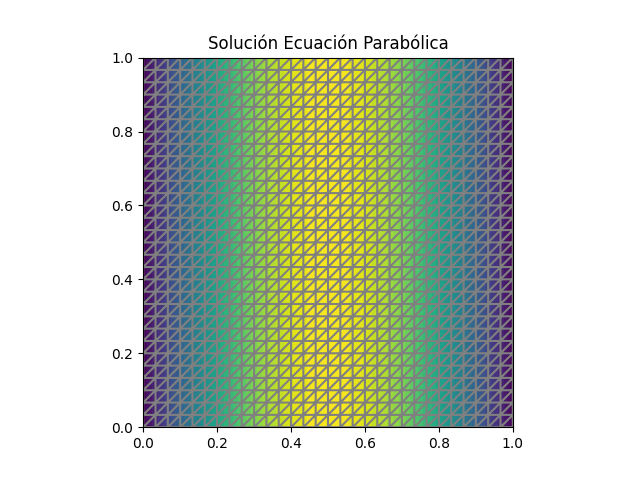
\includegraphics[scale=0.39]{../report/parabolic_FEniCS_mesh.png} 
\end{center} 
\caption{Tessellation used for the parabolic PDE}
\label{fig::parabolic_mesh}
\end{figure}




\subsection{Hyperbolic Equation}
The hyperbolic equation considered here is the wave equation. The problem is
\begin{equation} \label{eq::wave_equation}
\frac{\partial^2 u}{\partial t^2}(x,y)-4\frac{\partial ^2 u}{\partial x^2}(x,t)=0,\,\,\,0<x<1,\,\,\,t>0
\end{equation}
with boundary conditions
\begin{equation}
u(0,t)=u(1,t)=0,\,\,\, \text{for }\,\,t>0
\end{equation}
and initial conditions
\begin{equation}
u(x,0)=\sin(\pi x), \,\,\, \text{y}\,\,\,\frac{\partial u}{\partial t}(x,0)=0,\,\,\, 0\leq x \leq 1
\end{equation}
\subsubsection{Implementation in Mathematica}
The result of solving \ref{eq::wave_equation} with its boundary and initial conditions in Mathematica is shown below.
\begin{figure}[H]
\begin{center}
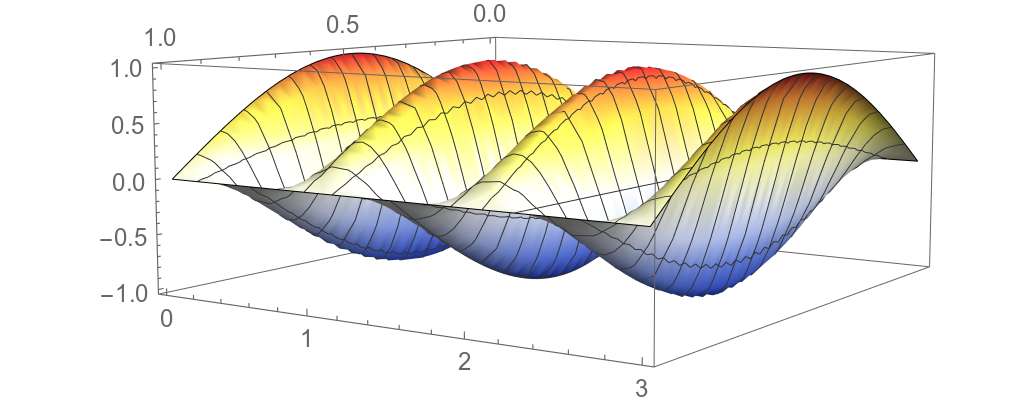
\includegraphics[scale=0.42]{../report/wave.png} 
\end{center} 
\caption{Numerical solution of the wave equation}
\label{fig::wave_mathematica}
\end{figure}
The corresponding contour lines are shown in the following figure.
\begin{figure}[H]
\begin{center}
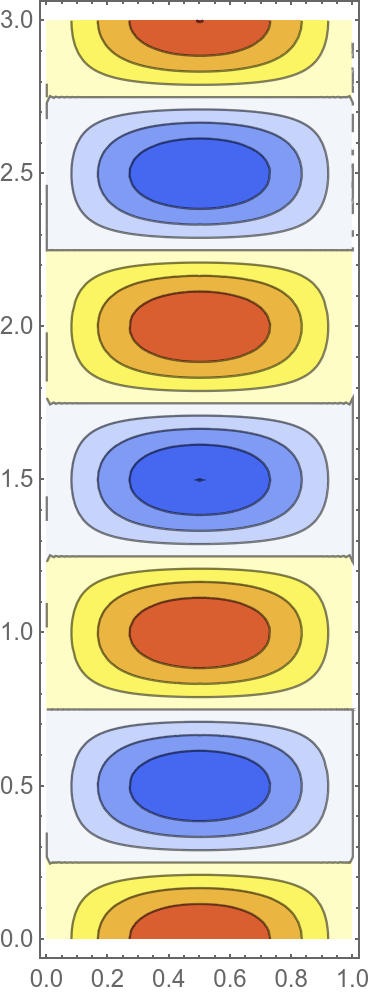
\includegraphics[scale=0.22]{../report/wave_contour.png} 
\end{center} 
\caption{Contour lines of the numerical wave-equation solution}
\label{fig::wave_contours}
\end{figure}
\subsubsection{Implementation in FEniCS}
Using the weak formulation of \ref{eq::wave_equation}, the problem can be treated with \texttt{FEniCS}. The result is shown below.
\begin{figure}[H]
%\begin{center}
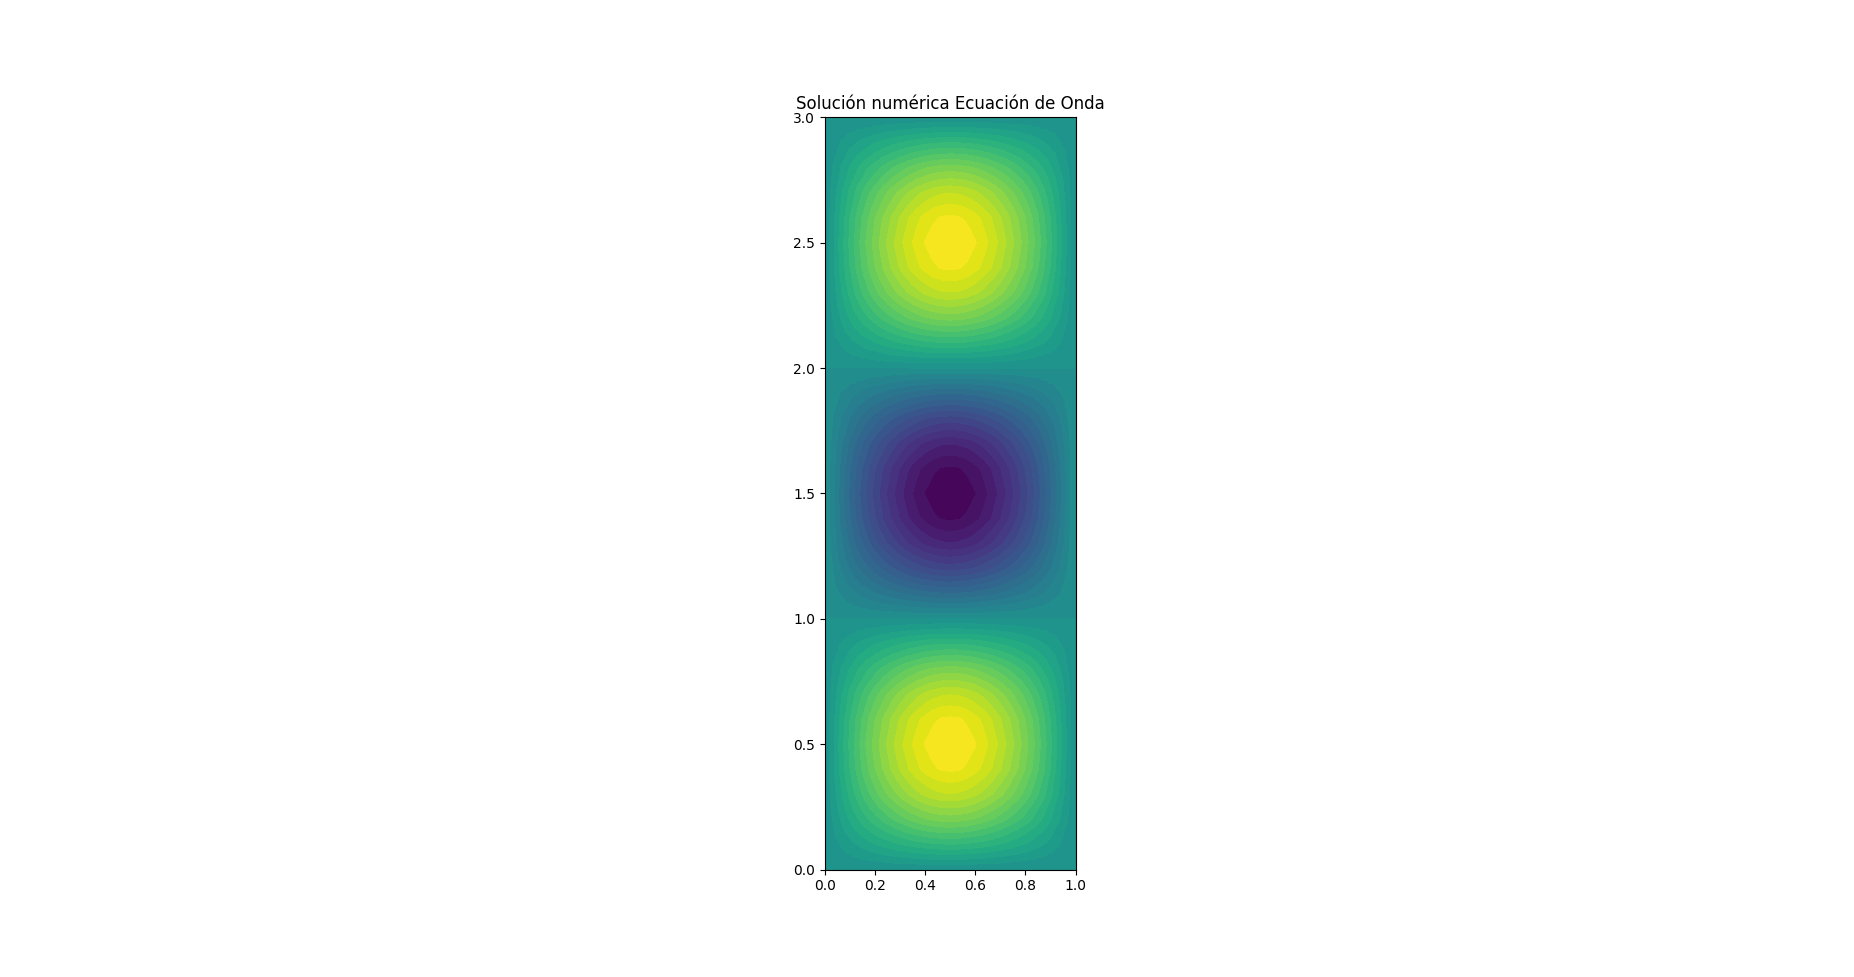
\includegraphics[scale=0.25, left]{../report/wave_FEniCS.png} 
%\end{center} 
\caption{Numerical solution of the wave equation}
\label{fig::wave_fenics}
\end{figure}
\section{Comparison of the Implementations}
To compare the implementations for the three canonical PDE classes, the average RAM consumption of each package was recorded.\\
\begin{center}
\begin{tabular}{ |c|c|c|c| } 
\hline
Partial Differential Equation & \texttt{Wolfram Mathematica}& \texttt{Python/FEniCS}\\
\hline
Elliptic& $188$ MB & $266$ MB \\
Parabolic& $178$ MB& $148$ MB\\
Hyperbolic& $178$ MB & $152$ MB\\
\hline
\end{tabular}
\end{center}
\subsection{Spatial Discretization}
Discretizing the domain is a fundamental step in the finite element method, and many theoretical approaches are available. As discussed previously, the choice of elementary geometric cell used for the tessellation directly affects the construction and quality of the method.\\

Some of the mesh-generation ideas associated with the \texttt{NDSolve`FEM`} framework in \texttt{Wolfram Mathematica} include the following:
\begin{enumerate}
  \item \textbf{Delaunay triangulation}: This is a common algorithm for generating two-dimensional meshes. A triangulation of a set of points is Delaunay if no point lies inside the circumcircle of any triangle. Delaunay triangulations tend to maximize the minimum triangle angle, producing comparatively well-shaped elements.
  \item \textbf{Voronoi diagram}: This is the geometric dual of a Delaunay triangulation. Given a set of points, each point is assigned a polygon containing the locations closer to that point than to any other. These polygons form a Voronoi diagram and can support mesh-refinement strategies.
  \item \textbf{Octree method (quadtree in 2D)}: The domain is divided recursively into eight equal parts in three dimensions, or four equal parts in two dimensions, until the desired resolution is reached. Specialized transition elements can connect regions with different levels of refinement.
  \item \textbf{Advancing-front method}: The procedure starts from a boundary mesh and progressively adds elements toward the interior. A front is maintained between meshed and unmeshed regions, and new nodes are introduced so that the front advances.
  \item \textbf{Ruppert\'s algorithm}: This is a Delaunay-refinement algorithm that also enforces a minimum-angle criterion, producing high-quality triangulations.
  

\end{enumerate}

\texttt{FEniCS} uses several related techniques and theoretical frameworks. As an open-source project, it also offers the following strengths:
\begin{enumerate}
  \item \textbf{Mesh generation}: FEniCS workflows can use libraries such as \texttt{mshr} and \texttt{CGAL} to create and manipulate complex meshes.
  \item \textbf{Automated finite element assembly}: A principal strength of \texttt{FEniCS} is its automated assembly of finite element systems. Variational forms, which provide the mathematical foundation of finite element discretization, can be expressed in notation close to the underlying mathematics directly in \texttt{Python} or \texttt{C++}.
  \item \textbf{Problem solution}: \texttt{FEniCS} uses \texttt{PETSc} to solve linear and nonlinear systems, providing powerful and scalable numerical solvers.
\end{enumerate}

\section{Statistical Analysis of Numerical Approximation Results}

Statistical analysis can be applied to the output of a numerical approximation to better understand the characteristics and performance of the method, validate the results, and draw inferences about the process that generated the data. Common techniques include:

\begin{enumerate}
  \item \textbf{Descriptive statistics}: The mean, median, mode, standard deviation, variance, range, minimum, maximum, quartiles, and related measures summarize the central tendency, dispersion, and distribution of the data.
  \item \textbf{Error analysis}: Residuals, defined as differences between observed and predicted values, can be calculated and their distribution examined. Metrics such as mean absolute error and mean squared error may be used, and residual plots can reveal systematic patterns.
  \item \textbf{Confidence intervals}: Confidence intervals around estimated parameters or predictions can be constructed to quantify uncertainty.
  \item \textbf{Hypothesis testing}: When a specific hypothesis is of interest, such as whether one approximation method outperforms another, an appropriate statistical test can be applied. For example, a $t$-test can compare the means of two groups.
  \item \textbf{Correlation analysis}: When several variables are present, their relationships can be examined with correlation coefficients or scatter plots.
  \item \textbf{Regression analysis}: When the results depend on multiple input variables, regression can help explain their collective influence and may also support prediction.
  \item \textbf{Analysis of variance (ANOVA)}: When comparing several approximation methods or several configurations of one method, ANOVA can assess whether the differences among groups are statistically significant.
  \item \textbf{Bootstrap or cross-validation}: Resampling or data-splitting techniques can be used to estimate the accuracy and stability of the approximation method.
  \item \textbf{Monte Carlo analysis}: If the numerical approximation involves randomness, as in Monte Carlo integration, the distribution of results over repeated runs can be analyzed through its mean, variance, and other statistical properties.
\end{enumerate}

\section{Conclusions}

The finite element method has become a fundamental tool in mathematical modeling, physical simulation, and engineering analysis. Partial differential equations subject to Dirichlet or Neumann boundary conditions are often difficult to solve analytically. A notable graduate-level example in physics is the study of electromagnetic boundary-value problems discussed by Jackson \cite{Jackson}.\\

Computational packages are therefore used throughout science, since most realistic problems do not admit closed-form analytical solutions. FEM is one of the most widely used numerical approaches in practice, particularly because of its ability to handle complex geometries and boundary conditions.\\

The results obtained for the three canonical PDE classes show that \texttt{Wolfram Mathematica} and \texttt{FEniCS} both provide robust and relatively accessible FEM implementations, each with advantages and disadvantages. Mathematica allows the problem to be formulated in a syntax close to ordinary mathematical notation: the PDE can be entered almost directly. FEniCS requires the user to derive and define the weak formulation explicitly. Mathematica is proprietary software, whereas FEniCS is open source, making FEniCS more accessible and configurable at the cost of requiring more detailed programming and numerical knowledge. For the examples considered here, the differences in RAM consumption are not substantial, although both Python and Mathematica are known to use significant memory.\\
With respect to execution time, Mathematica solved these examples almost immediately, whereas the Python implementation could require up to several minutes depending on the selected parameters. A future comparison with a \texttt{C++} implementation would provide a more informative performance benchmark.



\begin{thebibliography}{99}
%% The bibliography is ordered alphabetically by the surname of the
%% author or first author.
%% Each entry follows the format appropriate for a book, article,
%% thesis, website, or other source.


\bibitem{Burden} Richard L. Burden, J. Douglas Faires \textit{Numerical Analysis}, (Ninth Edition). Brooks/Cole, Cengage Learning. 978-0-538-73351-9

\bibitem{sfepy} Cimrman, R., Lukeš, V., Rohan, E., 2019. \textit{Multiscale finite element calculations in Python using SfePy}. Advances in Computational Mathematics 45, 1897-1921. https://doi.org/10.1007/s10444-019-09666-0

\bibitem{FEniCS}M. S. Alnaes, J. Blechta, J. Hake, A. Johansson, B. Kehlet, A. Logg, C. Richardson, J. Ring, M. E. Rognes and G. N. Wells.\textit{The FEniCS Project Version 1.5, Archive of Numerical Software 3 (2015)}. [doi.org/10.11588/ans.2015.100.20553]
\bibitem{}A. Logg, K.-A. Mardal, G. N. Wells. \textit{Automated Solution of Differential Equations by the Finite Element Method}, Springer(2012). [doi.org/10.1007/978-3-642-23099-8]

%\bibitem{Medina}Julio Medina. \textit{Finite Element Method}. \url{https://github.com/Julio-Medina/Finite_Element_Method}

\bibitem{Jackson}  John David Jackson. \textit{Classical Electrodynamics}. Wiley, 1999.
%\bibitem{Feynman} 
%\bibitem{Hopfield} J.J. Hopfield. \textit{Neural Networks and physical systems with emergent collective computational abilities}. \url{https://doi.org/10.1073/pnas.79.8.2554}


%\bibitem{McCulloch} Warren S. McChulloch, Walter H. Pitts. \textit{A LOGICAL CALCULUS OF THE IDEAS IMMANENT IN NERVOUS ACTIVITY}. \url{http://www.cse.chalmers.se/~coquand/AUTOMATA/mcp.pdf}



\end{thebibliography}
\end{document}

